\section{Higher-dimensional tower topology}\label{sec:towertop}
The two towers of \cref{sec:towers} give, for each $k$, an occurrence set $D_k=D(x_k)$ and a complex $K_k=K(D_k)$ with $x_k=S_k^2/m$ ($m=11$, $S_k=2^23^{3+k}5^4$, or $m=5$, $S_k=126\cdot2^k$). We study $k\mapsto\beta_i(K_k)$. Four statements are kept apart throughout: the \emph{existence} of an eventual quasi-polynomial law, its \emph{period}, an \emph{effective threshold} after which it holds, and \emph{exact formulas} for the Betti numbers. Only the first two are proved here for all $k$; the last two are finite-exact.

\subsection{Towers are nested filtrations}
\begin{theorem}[nested tower]\label{thm:A5T51}
For $k\le k'$ on either tower: (a) $D_k=\{d\in D_{k'}:d\mid S_k\}$; (b) $K_k$ is the induced subcomplex of $K_{k'}$ on the vertices $D_k$ (the cells of $K_{k'}$ all of whose vertices lie in $D_k$); in particular $K_k\subseteq K_{k+1}\subseteq\cdots$; (c) at every event of the orbit, $x_{8k+7}\to x_{8k+8}$ (resp.\ $x_{3k+2}\to x_{3k+3}$), no cell dies: $\mathrm{Dead}=\emptyset$.
\end{theorem}
\prov{CW-0448}{A5-T5.1}{PROVED}{FULL}
\begin{proof}
(a) $D_k=\{d\mid S_k:d\ge2,\ d\equiv1\ (m)\}$ and $S_k\mid S_{k'}$. (b) For $u,v\in D_k$ every element of $[u,v]^\circ$ divides $\lcm(u,v)\mid S_k$, so $[u,v]^\circ\cap(D_{k'}\cup\{1\})=[u,v]^\circ\cap(D_k\cup\{1\})$ by (a). By \cref{thm:A5T31} $K(D_k)$ and $K(D_{k'})$ have the same edges among $D_k$, hence the same cells with all vertices in $D_k$ (cells are determined by their vertices and $1$-faces). (c) By \cref{thm:R3T5bp,thm:R3T5c} the orbit between $x_{\cdot}$ and the event has $D=D_k$ and then $D=D_{k+1}$; the new occurrences $N=D_{k+1}\setminus D_k$ do not divide $S_k$ and every interval of an edge of $K_k$ consists of divisors of $S_k$, so no edge is pierced (\cref{thm:A5T32}(2)). \qedhere
\end{proof}
\begin{remark}[consequence for homology]
By \cref{thm:cause} and \cref{thm:nested}, along a tower a Betti number is created as relative homology of the new slab and can only be lowered by new cells of one higher dimension. This is why the two towers, which have the same structural form, differ only through the cross-section (the caps of the fixed primes and the lattice $\Lambda$), not through any piercing.
\end{remark}
The nested filtration is drawn in \cref{fig:nestedtowers}.
\begin{figure}[tbp]\centering
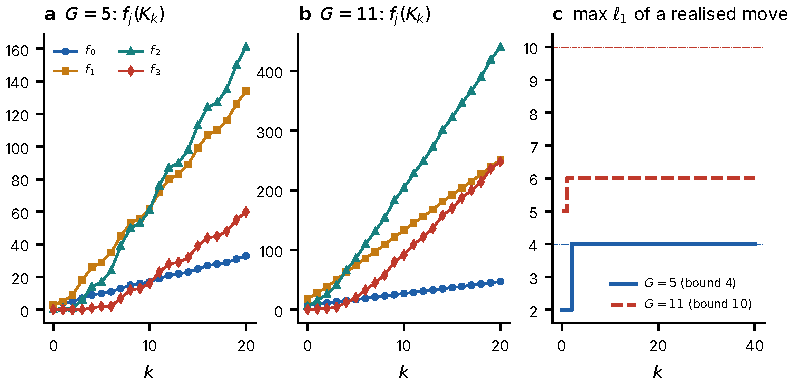
\includegraphics[width=\textwidth]{fig25_nested_towers}
\caption{\textbf{Nested towers (finite-exact; nestedness proved by \cref{thm:A5T51}).} (a), (b) $f$-vectors of $K_k$ for the $G=5$ and $G=11$ towers, $k\le20$ (shown range). (c) Largest $\ell_1$-norm of a realised move for $k\le40$: at most $4$ for $G=5$ and $6$ for $G=11$, below the proved bounds $4$ and $10$ of \cref{lem:A5T52}. Inclusion of cell sets $K_k\subseteq K_{k+1}$ was also verified for all $k\le25$ (both towers). Nothing beyond the computed range is plotted.}\label{fig:nestedtowers}
\end{figure}

\subsection{Stabilisation of moves and the qualitative Betti law}
\begin{lemma}[moves stabilise]\label{lem:A5T52}
Let $\Lambda=\ker(\Z^r\to(\Z/m)^*,\ g\mapsto\prod p_i^{g_i})$ for the primes $p_i$ of $S_k$. Every region-Graver vector $g$ satisfies $\|g\|_1\le|\langle p_1,\dots,p_r\rangle|\le\varphi(m)$. Hence all moves of the towers have $\ell_1$-norm at most $10$ ($m=11$) resp.\ $4$ ($m=5$), and once the cap of the growing prime exceeds this bound the set of moves of $K_k$ does not change with $k$.
\end{lemma}
\prov{CW-0449}{A5-T5.2}{PROVED}{FULL}
\begin{proof}
A region-Graver vector is minimal in $\Lambda\cap[-q,q]$; every $h\sqsubseteq g$ lies in the box, so $g$ is a Graver vector of $\Lambda$. Because $g$ has a fixed sign in each coordinate, $g$ is the sequence $a_1,\dots,a_n$ ($n=\|g\|_1$) consisting of $g_i^+$ copies of $p_i$ and $g_i^-$ copies of $p_i^{-1}$ in the group $H=\langle p_i\rangle\le(\Z/m)^*$, with product $1$, and minimality says that it has no proper non-empty zero-sum sub-sequence. The partial products $s_j=a_1\cdots a_j$ ($1\le j\le n-1$) are $\ne1$ (a prefix would be a zero-sum subsequence) and pairwise distinct (a quotient $s_j/s_i$ would be one), so $n-1\le|H|-1$. For $m$ prime $\varphi(m)=m-1$. \qedhere
\end{proof}
\begin{theorem}[eventual quasi-polynomial Betti laws, qualitative]\label{thm:A5T53}
Let $\rho$ be the growing prime ($\rho=3$, $m=11$; $\rho=2$, $m=5$), $\omega=\ord_m(\rho)$ ($\omega=5$, resp.\ $4$). For every field $\mathbb k$ and every $i\ge0$ there exist an integer $k_1$ and a quasi-polynomial $q_i$ of degree $\le1$ and period dividing $\omega$ such that $\beta_i(K_k;\mathbb k)=q_i(k)$ for all $k\ge k_1$. The threshold $k_1$ is \emph{not} controlled.
\end{theorem}
\prov{CW-0450}{A5-T5.3}{PROVED-SCOPED}{SPLIT}
\begin{proof}[Proof (structure; the threshold is not effective)]
Use the coordinates $(u,h)\in\Z^{r-1}\times\Z$ with $h$ the exponent of $\rho$, and let $\Lambda'$ be the lattice. Let $\tilde K$ be the complex defined by the interval rule on the infinite slab $\Lambda'\cap(\text{box}\times\N)$ \emph{including the origin as a vertex}; $K_k$ is the subcomplex of cells avoiding the origin and of height $\le h_0+k$ (an edge between non-origin vertices has an interval of lower height, so the rule is the same). Since $\rho^\omega\equiv1$, the shift $T:(u,h)\mapsto(u,h+\omega)$ preserves $\Lambda'$, and the lattice points of the shifted box are the shifts of those of the box, so $T$ is an injective cellular map; a cell whose minimal height is at least $\omega$ is the image under $T$ of a cell of $\tilde K$ (if the preimage box meets the origin, $T$ of the origin is a lattice point of the shifted box, so the origin is then a vertex of the preimage cell). By \cref{lem:A5T52} cells have bounded diameter, hence the cells of $\tilde K$ that are not in the image of $T$ form a finite set. Form $R=\bigoplus_hC_*(K_h)$ as a graded module over $\mathbb k[t,T]$, $t$ acting by inclusion $K_h\to K_{h+1}$ (degree $1$) and $T$ by the shift (degree $\omega$); it is finitely generated by the above finite set of cells (and the shifts of the finitely many cells through the origin). By Noetherianity $\bigoplus_hH_i(K_h)=H_i(R)$ is a finitely generated graded module, and the Hilbert function of a finitely generated graded module over $\mathbb k[t,T]$ with weights $(1,\omega)$ is eventually a quasi-polynomial of degree $\le1$ and period dividing $\omega$ (Hilbert--Serre; \cite{Eisenbud1995}; for quasi-polynomials in this form \cite{Stanley1997,Ehrhart1962}). \qedhere
\end{proof}
\begin{corollary}[conditional exact formulas]\label{cor:cond}
If for the $G=11$ tower the regime of $\beta_1$ (resp.\ $\beta_2$, $\beta_3$) begins at some $k_1\le130$, then $\beta_1\equiv8$ and $\beta_2\equiv17$ for all $k\ge k_1$, resp.\ $\beta_3(k+5)=\beta_3(k)+9$ for all $k\ge\max(k_1,8)$. The unconditional statement needs a bound on $k_1$ (a regularity bound for the module $H_i(R)$), which is open.
\end{corollary}
\begin{proof}
A quasi-polynomial of degree $\le1$ and period $5$ is determined by two values in each residue class. Between $k_1$ and $140$ there are at least $10$ computed consecutive values, in each residue class at least two, on which the computed laws of \cref{thm:A5T6} hold. \qedhere
\end{proof}
\begin{remark}[four distinctions]
(i) \emph{Existence} of an eventual quasi-polynomial: proved (\cref{thm:A5T53}). (ii) \emph{Period}: divides $\omega$: proved. (iii) \emph{Effective threshold} $k_1$: not known; the observed onset ($k=2$ for $\beta_1$, $k=6$ for $\beta_2$, $k=8$ for $\beta_3$ on $G=11$; $k=7$ on $G=5$) is a computed fact for $k\le140$. (iv) \emph{Exact formulas}: finite-exact to $k\le140$, and exact for all $k$ only under the hypothesis of \cref{cor:cond}. The formulas are not promoted to universal ones.
\end{remark}

\subsection{Contrast: corrected \texorpdfstring{$\sigma$}{sigma}-transport versus collective monotonicity}\label{ssec:contrast}
The \emph{collective} map is monotone: $D(x)\subseteq D(C(x))$ (\cref{lem:M}), so occurrences persist and the complex only changes by the transition law. The \emph{generative} SELECT-II edges $m\xrightarrow{N}m'=m(N+1)^2/N$ ($N\mid m$) behave differently, and the claim of inclusion for them must not be carried over.
\begin{proposition}[corrected $\sigma$-transport, B2-T9]\label{prop:B2T9}
On every SELECT-II edge $\sigma(m')=\sigma(m)(N+1)/c$ with $c=\prod_{p\mid N}p^{l_p}$ and $c\le N$. Hence $\sigma$ \emph{strictly increases}, $\sigma(m')>\sigma(m)$, and $D(m')\ne D(m)$ (since $\sigma=\max D$): no step is silent. It is \emph{not} true that $D(m)\subseteq D(m')$ or that $\sigma(m)\mid\sigma(m')$: the edge $4\xrightarrow{2}18$ has $D(4)=\{2\}$, $D(18)=\{3\}$.
\end{proposition}
\prov{CW-0403}{B2-T9}{CORRECTED}{CORRECTED}
\begin{proof}
The transport formula is \cref{thm:B2T2}. Since $l_p\le v_p(N)$, $c\le N<N+1$. For the example: $4=2^2$ has $\sigma=2$; $18=2\cdot3^2$ has $\sigma=3$. \qedhere
\end{proof}
\begin{remark}[finite-exact check]
On all $24{,}496$ edges with $1\le m\le3000$, $N\mid m$: the transport formula holds, $\sigma$ strictly increases and $D$ changes on every edge; the inclusion $D(m)\subseteq D(m')$ holds on $13{,}894$ edges and fails on $10{,}602$ (the first failure is $m=4$, $N=2$). A table of the $24{,}495$ edges with $m\ge2$ in the inherited note differs from this count only by the edge $1\to4$ (\stat{finite-exact}). Nothing in this paper uses inclusion on generative edges, and no Graver-basis monotonicity claim is made.
\end{remark}
\begin{remark}[what this does to the comparison]
The contrast is part of why the hierarchy of \cref{sec:corr} is kept level by level: a statement that holds along collective orbits (persistence of occurrences, nested towers) need not hold along generative histories.
\end{remark}

\subsection{Exact tower laws to \texorpdfstring{$k\le140$}{k<=140}}\label{ssec:towerlaws}
\begin{theorem}[tower laws; finite-exact]\label{thm:A5T6}
The following were computed exactly (over $\mathbb F_2$ and over $\mathbb F_p$, $p=2^{31}-1$, which gave the same Betti vector at every $k$) for every $k\le140$ and are \emph{not} extrapolated.
\begin{enumerate}[label=(\alph*),itemsep=1pt]
\sloppy\item $G=11$: $\beta_0=1$; $\beta_1=6,7,8,8,8,\dots$ ($=8$ for $2\le k\le140$); $\beta_2=0,1,4,7,13,16,17,17,\dots$ ($=17$ for $6\le k\le140$); $\beta_3=0$ for $k\le8$ and $\beta_3(k+5)=\beta_3(k)+9$ for $8\le k\le135$, with $(\beta_3(8),\dots,\beta_3(12))=(0,4,4,7,8)$; $\beta_4=0$. Moreover $|D_k|=2k+7$ (proved, \cref{thm:R3T5bp}).
\item $G=5$: $(\beta_0,\beta_1,\beta_2,\beta_3)=(1,1,0,0),\allowbreak(1,1,0,0),\allowbreak(1,4,0,0),\allowbreak(1,6,0,0),\allowbreak(1,6,1,0),\allowbreak(1,6,1,0),\allowbreak(1,6,3,0)$ for $k=0,\dots,6$ and $(1,6,5,0)$ for every $7\le k\le140$.
\item The event at the orbit step $5\to6$ of the $G=5$ tower, which is the tower-index step $k=1\to2$ (not ``$5\to6$'' in the index $k$), adds one occurrence ($56$), four new edges to old vertices, no dead cell and no new $2$-cell, $f=(4,5,1)\to(5,9,1)$, and $\beta_1$ passes from $1$ to $4$; this is the star formula $\Delta\beta_1=4-1=3$ of \cref{thm:A5T44}.
\end{enumerate}
\end{theorem}
\prov{CW-0451}{A5-T6}{FINITE-EXACT}{FINITE}
\begin{proof}[Computation]
Both towers were generated from the closed forms of \cref{thm:R3T5bp,thm:R3T5c}, the complexes $K(D_k)$ were built with the interval rule and the Betti numbers computed by exact linear algebra over both fields, with the check $\partial^2=0$ over $\F_2$ at every $k$; the closed forms for $|D_k|$ were checked at every $k$. The full tables are in Appendix~\ref{app:towers}. \qedhere
\end{proof}
The computed Betti numbers of the two towers are plotted in \cref{fig:g5betti,fig:g11betti}.
\begin{figure}[tbp]\centering
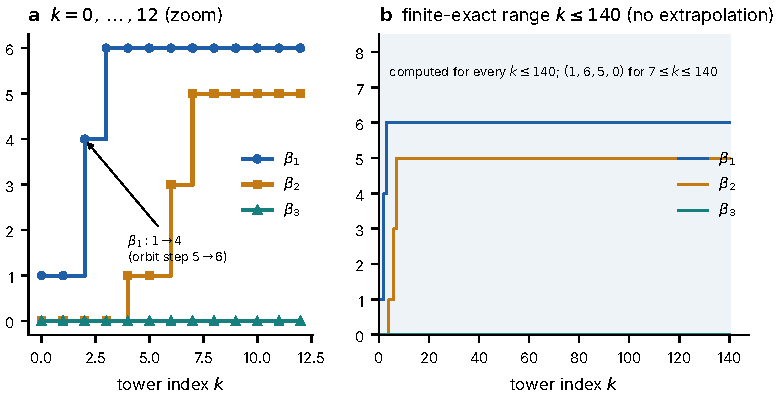
\includegraphics[width=\textwidth]{fig23_g5_betti}
\caption{\textbf{Betti numbers of the $G=5$ tower (finite-exact; \cref{thm:A5T6}).} $S_k=126\cdot2^k$. (a) $\beta_1,\beta_2,\beta_3$ for $k=0,\dots,12$; the jump $\beta_1:1\to4$ is at tower index $k=1\to2$ (orbit step $5\to6$). (b) the whole computed range $k\le140$ (shaded); the values $(1,6,5,0)$ hold for every computed $7\le k\le140$. No curve is extended beyond $k=140$.}\label{fig:g5betti}
\end{figure}
\begin{figure}[tbp]\centering
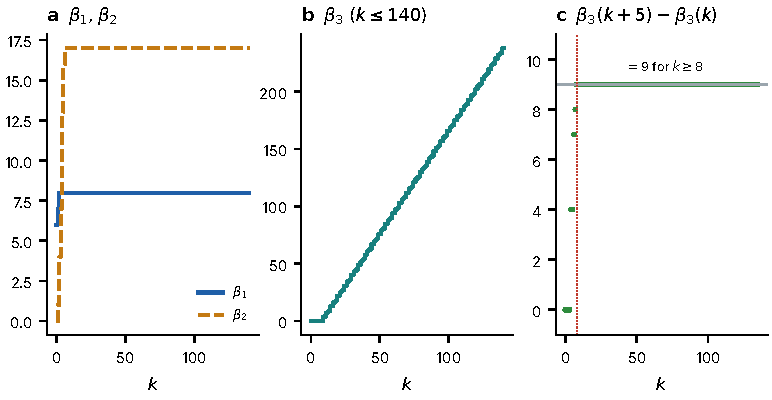
\includegraphics[width=\textwidth]{fig24_g11_betti}
\caption{\textbf{Betti numbers of the $G=11$ tower (finite-exact; \cref{thm:A5T6}).} $S_k=2^2\,3^{3+k}\,5^4$, computed for every $k\le140$. (a) $\beta_1,\beta_2$ (stable at $8$ and $17$). (b) $\beta_3$. (c) the increment $\beta_3(k+5)-\beta_3(k)$, equal to $9$ for all computed $k\ge8$. The periodic structure of period $5$ is that of $\ord_{11}(3)=5$ (a proved arithmetic fact), the values are computed.}\label{fig:g11betti}
\end{figure}
\begin{proposition}[comparison of the two towers; finite-exact and open]\label{prop:A4T56}
Both towers are nested with $\mathrm{Dead}=\emptyset$ (\cref{thm:A5T51}) and have exactly one occurrence event per period, but the Betti vectors differ: $G=5$ is bounded with $\beta_3=0$, $G=11$ has $\beta_3$ growing linearly in $k$ over the computed range. The scaling laws $x_{n+3}=4x_n$ and $x_{n+8}=9x_n$ determine $D$ and hence the realised complex, but not the dormant relations and not the Betti pattern; the stabilisation scale is set by the Graver bound ($4$ versus $10$) and by $\omega$ ($4$ versus $5$) (\cref{lem:A5T52,thm:A5T53}). \emph{No theorem here explains why $G=11$ has growing $\beta_3$ while $G=5$ has none}; this is open (\cref{sec:concl}). The $\ell=29$ tower stays finite-exact (\cref{ex:l29}).
\end{proposition}
\prov{CW-0434}{A4-T5}{MIXED}{SPLIT}
\prov{CW-0435}{A4-T6}{FINITE-EXACT}{FINITE}
